\documentclass[paper=a4,fontsize=11,parskip=full,pagesize=auto,BCOR=5mm,DIV=12]{scrbook}

\usepackage[english]{babel}
\usepackage[T1]{fontenc}
\usepackage{lmodern}
\usepackage{microtype}
\usepackage{csquotes}
\usepackage[style=ieee,dashed=false,url=false,eprint=false]{biblatex}
\usepackage{listings}
\usepackage[dvipsnames]{xcolor}
\usepackage{inconsolata}
\usepackage{booktabs}
\usepackage{graphicx}
\usepackage{float}
\usepackage{adjustbox}
\usepackage[printsolution=true]{exercises}
\usepackage{scrhack}
\usepackage[shortlabels]{enumitem}
\usepackage{pifont}
\usepackage{makecell}
\usepackage{dsfont}
\usepackage{mathtools}
\usepackage{algorithm}
\usepackage{algorithmicx}
\usepackage{algpseudocode}
\usepackage{threeparttable}
\usepackage{tkz-graph}
\usepackage{collcell}
\usepackage{tabularx}
\usepackage{hyperref}
\usepackage{todonotes}
\usepackage{menukeys}

\lstset{
    language = java,
    captionpos = t,
    basicstyle = \ttfamily\footnotesize,
    keywordstyle = \color{blue},
    commentstyle = \color{gray},
    stringstyle = \color{red},
    columns = fullflexible,
    breaklines = true,
    frame = single,
    numbers = left,
    numberstyle = \scriptsize\sffamily\color{gray},
    xleftmargin = 0.08\textwidth,
    xrightmargin = 0.08\textwidth,
    showstringspaces = false,
    float
}

\renewcommand\theadfont{\bfseries}
\newcommand{\cmark}{\ding{51}}
\newcommand{\xmark}{\ding{55}}
\addbibresource{references.bib}
\def\CC{{C\nolinebreak[4]\hspace{-.05em}\raisebox{.4ex}{\tiny\normalfont\bfseries ++}}}
\algnewcommand{\Raise}{\State\textbf{raise }}
\newcommand{\includepic}[1]{\includegraphics[width=3.5cm,keepaspectratio]{images/#1}}
\newcolumntype{i}{@{\hspace{1ex}}>{\collectcell\includepic}c<{\endcollectcell}}

\begin{document}
    \titlehead{Atılım University\\Department of Software Engineering}
    \title{System Software Validation and Testing Lab Manual}
    \author{Tolga Üstünkök\thanks{E-mail: tolga.ustunkok@atilim.edu.tr} \and Ali Yazıcı\thanks{E-mail: ali.yazici@atilim.edu.tr}}
    \date{January 2022}
    \publishers{Department of Software Engineering\\Atılım University}
    \lowertitleback{This lab manual was set with the help of {\KOMAScript} and {\LaTeX} and last compiled on {\today}. The document source can be found in \url{https://github.com/tustunkok/se344-lab-manual}.}
    \maketitle
    
    \frontmatter
    \tableofcontents
    \listoffigures
    \listoftables
    \lstlistoflistings
    \listoftodos
    
    \mainmatter
    \chapter{Introduction}
\label{ch:introduction}
Software testing and test design is very important and inseparable part of the software development process. The application of testing methods is as important as the theory of testing. This manual aims to be a supplementary document to the theoretical lectures of software testing. It can be used as an introductory guide to JUnit Jupiter API or can be followed as a text for laboratory studies. Java is chosen as the primary programming language for the exercises. Each section has two essential parts; the first one introduces the focused subject and the second one presents some exercises on the subject. Sections are designed to cover a 10-weeks semester schedule. However, some sections can be taught as two-week sections.

\section{Brief Introduction to Java Programming Language}
Java is an object-oriented programming language created by Sun engineers James Gosling, Mike Sheridan, and Patrick Naughton in 1991. Java programs are compiled into a special bytecode before being interpreted by Java Virtual Machine (JVM). This bytecode can be thought of as a high-level version of low-level machine languages such as Assembly. JVM interprets the bytecode and makes the system calls and other necessary operations on behalf of the running bytecode. This additional layer sometimes causes Java programs to be a little bit slower than their C/\CC~counterparts. Because of this "compilation then interpretation" stage Java can be classified as a hybrid programming language. 

One advantage of using a JVM is that every operating system has its own implementation of JVM. Therefore, the same Java program can be run in multiple operating systems without any change in the code. This is why Java is known as a platform-independent language.

\subsection{Java Terminology}
Before moving on to more complex topics, let's discuss the most common terminology of Java. Some of the below terms are discussed before and some are new.

\begin{enumerate}
    \item \textbf{Java Virtual Machine (JVM):} A written program is first converted to a low-level language called bytecode by a program called \emph{javac}. Then, JVM interprets the bytecode and makes the operation on behalf of it.
    
    \item \textbf{Bytecode:} As discussed previously, it is a low-level language model to communicate with JVM. It can be physically found in projects as files with \emph{.class} file extension.
    
    \item \textbf{Java Development Kit (JDK):} JDK is a complete development environment to develop Java programs. It contains a compiler, Java Runtime Environment (JRE), Java debuggers, Java documentations, etc.
    
    \item \textbf{Java Runtime Environment (JRE):} JRE is just an environment only capable of running pre-compiled Java programs. One cannot compile Java programs with only JRE installed. JRE includes a browser, JVM, applet supports, and plugins. To be able to run a Java program a computer should have at least JRE installed on it.
    
    \item \textbf{Garbage Collector:} Unlike C/\CC, one cannot delete objects manually in Java. This responsibility is taken care of automatically by a special program called \emph{Garbage Collector}. Garbage collector detects the objects which have not been referenced anymore and deletes them to recollect the memory occupied by them.
    
    \item \textbf{ClassPath:} The classpath is the file path where the Java runtime and Java compiler look for .class files to load. If you want to add external libraries , then you must add them to the classpath.
\end{enumerate}

\subsection{An Overview of a Hello World Program}
Java has many features. Some of them are object-oriented, multithreaded, allows sandbox execution, and the list goes on. Curious readers can find the full list on GeeksForGeeks website\footnote{\url{https://www.geeksforgeeks.org/introduction-to-java/?ref=lbp}}.

The best way to explain some syntax rules is to go through an example. Let's look at the example Java program shown in Listing \ref{lst:java-hello}.

\begin{lstlisting}[caption={Hello world example written in Java.},label=lst:java-hello]
// Demo Java program

// Importing classes from packages
import java.io.*;

// Main class
public class SomeClassName {
    // Main driver method
    public static void main(String[] args) {

        // Print statement
        System.out.println("Hello World!");
    }
}
\end{lstlisting}

The lines starting with \lstinline!//! are called \emph{comment} lines. Compilers ignore the comment lines. Comments can be single line or multiple lines. Multiple line comments start with \verb|/*| and end with \verb|*/|. e.g. \verb|/* A multiline comment */|.

The line \lstinline!import java.io.*;! means that import all the classes of \lstinline!io! package which also belongs to another package called \lstinline!java!. This is generally \textbf{not} a recommended way of importing packages.

Following the import statement, \lstinline!public class SomeClassName! defines a class. Here, \lstinline!public! is an \emph{access modifier}. It defines the places that can access to this class. Then, keyword \lstinline!class! indicates that we are defining a class with the name \lstinline!SomeClassName!. In Java, each file can have only one class (except for the inner classes) and the name of the class and the file that holds the class must be the same. Otherwise, Java compiler raises an error.

Each Java program starts from a \lstinline!static! method called \lstinline|main| which takes a \lstinline|String| array for command-line arguments. This method must be \lstinline|static| because it does not actually belong to the class which defines it and must be called externally by the JVM. In Listing \ref{lst:java-hello}, this method is defined as \lstinline!public static void main(String[] args)!. Here, the access modifier is set to \lstinline|public|. However, it is not necessary. Followed by the \lstinline|static|, the return type of the method is set to \lstinline|void|. This means that the method returns nothing after it is called which makes sense.

In Java, writing and reading operations always work on streams. In this case, by writing \lstinline{System.out.println("Hello world!");} we want to get the \lstinline|System.out| stream which is \lstinline|stdout| pseudo-file (console) and print a newline character terminated string. We can also get the \lstinline|stdin| pseudo-file to be able to read the inputs from the console by utilizing the \lstinline|System.in|.

You are now ready to expand your knowledge about Java further with this basic Java introduction. Some important resources to learn Java are \autocite{schildt2007java,schildt2010java,horstmann_2021}.

\section{Dependency Management with Maven}
Dependency management is a big part of every software development especially if multiple dependencies are involved. Each dependency can also depend on other dependencies and their specific versions. This is a huge problem because sometimes developers need to use an incompatible version as a dependency of the software they are developing which is a dependency of another dependency. These types of problems are hard to solve by humans. Because of this, various helper programs can be used. One of them is Maven, another popular one is Gradle. The list can be long for popular programming languages such as Java.

In this lab, we are going to focus on Maven. Without saying much, one can reach all the detailed information about Maven on Apache Maven Project website\footnote{\url{https://maven.apache.org/guides/getting-started/index.html}}. Let's return to the subject. Each Maven project has the same directory structure shown in Table \ref{tab:maven-dir-layout}.

\begin{table}
    \centering
    \renewcommand{\arraystretch}{1.2}
    \caption{Maven directory layout.}
    \label{tab:maven-dir-layout}
    \begin{tabular}{ll}
        \toprule
        Directory/File & Description \\
        \midrule
        \directory{src/main/java} & Application/Library sources \\
        \directory{src/main/resources} & Application/Library resources \\
        \directory{src/test/java} & Test sources \\
        \directory{src/test/resources} & Test resources \\
        \verb|target| & Output of the build \\
        \verb|pom.xml| & Description of the project \\
        \bottomrule
    \end{tabular}
\end{table}

There can be other directories in the project. A full list can be found in Apache Maven Project website\footnote{\url{https://bit.ly/34VlPvC}}. The \directory{src} directory holds the source code of the software and other resources such as images, database files, etc. The \directory{target} directory contains the output of a build. The most important file for a Maven project is the \lstinline[language={}]|pom.txt| file. This file is an Extensible Markup Language (XML) file to hold all the necessary information about the project and its dependencies. An example \lstinline[language={}]|pom.xml| file is shown in Listing \ref{lst:pom-example}.

\begin{lstlisting}[language=XML,caption={An example pom.xml file.},label=lst:pom-example]
<project xmlns="http://maven.apache.org/POM/4.0.0" xmlns:xsi="http://www.w3.org/2001/XMLSchema-instance" xsi:schemaLocation="http://maven.apache.org/POM/4.0.0 http://maven.apache.org/xsd/maven-4.0.0.xsd">
    <modelVersion>4.0.0</modelVersion>
 
    <groupId>com.mycompany.app</groupId>
    <artifactId>my-app</artifactId>
    <version>1</version>
    
    <properties>
        <mavenVersion>3.0</mavenVersion>
    </properties>
 
    <dependencies>
        <dependency>
            <groupId>org.apache.maven</groupId>
            <artifactId>maven-artifact</artifactId>
            <version>${mavenVersion}</version>
        </dependency>
        <dependency>
            <groupId>org.apache.maven</groupId>
            <artifactId>maven-core</artifactId>
            <version>${mavenVersion}</version>
        </dependency>
    </dependencies>
</project>
\end{lstlisting}

Each \lstinline[language={}]|pom.xml| file is actually an XML Schema Definition (XSD). At the top level, a project element defines the namespace information in its attributes. In the subelements, the version of the project, group id, artifact id, and properties are declared. Following the properties, a complex element called \lstinline[language={XML}]|<dependencies>| declares the dependencies of the project. There is a wide variety of elements to use inside the project. Full list can be obtained from here\footnote{\url{https://maven.apache.org/pom.html}}.

\section{Installing Eclipse and Setting Up a Maven Project}
Fortunately, most of the time we do not have to deal with constructing the directory structure or writing the \lstinline[language={}]|pom.xml| file. Most Integrated Development Environments (IDE) prepare those structures with project creation wizards and automate the building tasks. You can write Java code even in the simple Notepad program. However, using an IDE greatly reduces the overhead of building and writing software. There are many great choices when it comes to IDEs. In this manual, Eclipse IDE is chosen. To install Eclipse in Windows, just go to the official website\footnote{\url{https://www.eclipse.org/downloads/}} and download the download manager and install Eclipse for Java. For Linux, just use the package manager of the distribution that you are using. Notice that, it is assumed that either OpenJDK or Oracle JDK has been already installed in your computer. Alternatively, you can install Eclipse independently from the distribution via Snap\footnote{\url{https://snapcraft.io/store}} in Linux or via Chocolatey\footnote{\url{https://community.chocolatey.org/packages}} in Windows 10 or above.

After installing Eclipse, a standard welcome screen should be opened as shown in Figure \ref{fig:eclipse-welcome}. In this screen, close the welcome tab and go to \menu{File > New > Project...}.

\begin{figure}[H]
    \centering
    \includegraphics[width=0.95\textwidth]{images/eclipse-welcome.png}
    \caption{Welcome screen of Eclipse.}
    \label{fig:eclipse-welcome}
\end{figure}

A new dialog window should be showing up as in Figure \ref{fig:eclipse-project}. Search and choose the \emph{Maven Project}. After that, a wizard (shown in Figure \ref{fig:maven-new}) asks you a few questions about how you want to configure your new project.

\begin{figure}[H]
    \centering
    \includegraphics[width=\textwidth]{images/eclipse-project.png}
    \caption{Create a new project window.}
    \label{fig:eclipse-project}
\end{figure}

In Figure \ref{fig:maven-new}, make sure that \emph{Create a simple project} checkbox is checked. This will allow us to skip some unnecessary configuration options in the next pages. Click \keys{Next >} and you should see the dialog window shown in Figure \ref{fig:maven-app-conf}.

\begin{figure}[H]
    \centering
    \includegraphics[width=\textwidth]{images/maven-new.png}
    \caption{Maven project wizard landing page.}
    \label{fig:maven-new}
\end{figure}

In Figure \ref{fig:maven-app-conf}, there are only two fields that must be filled before clicking to the \keys{Finish} button. The first one is the \emph{Group Id} field. Here, you should write a general package name that normally should hold all of your similar projects. For example, since we are going to write a project specifically for the SE344 lab that is offered at Atılım University, we can write something like this: \lstinline|edu.atilim.se344|. The first part, \lstinline|edu|, indicates the top-level domain as on the Internet. Then, it is followed by the company name; in this case, it is our university. Finally, followed by the name of the course. In \emph{Artifact Id}, we just give a name to our build target/executable. In this case, it is \lstinline|lab1|. When we build the project, our build target will be named like \lstinline[language={}]|lab1-0.0.1-SNAPSHOT.jar|. When you have finished filling the necessary fields, click \keys{Finish} button. The new project should be created.

\begin{figure}[H]
    \centering
    \includegraphics[width=\textwidth]{images/maven-app-conf.png}
    \caption{Maven project wizard final page.}
    \label{fig:maven-app-conf}
\end{figure}

Before moving on to the next topic, there is a small problem that we need to address. In some versions of Eclipse, Java projects have a default Java version of 1.5. This is a problem for us. Therefore, right-click to the newly created project and click \menu{Properties}. The dialog window shown in Figure \ref{fig:java-version} should be opened. Here, click \emph{Java Compiler} in the list view. Untick the checkbox starting \emph{Use compliance from execution...} and select 1.8 from \emph{Compiler compliance level} checkbox. Click \keys{Apply \& Close} button when you have finished with the project properties.

\begin{figure}[H]
    \centering
    \includegraphics[width=\textwidth]{images/java-version.png}
    \caption{Java compiler properties for a Java project.}
    \label{fig:java-version}
\end{figure}

This concludes our project creation step. Now, we need to add necessary dependencies to our project's \lstinline[language={}]|pom.xml| file. In this case, there is only one dependency\todo{There are multiple dependencies.} and it is JUnit Jupiter API. In the next section, we are going to see how to add such dependencies to our project. Also, we need to make sure that our Maven build system is compatible with JUnit. We will add a plugin to our project to comply with JUnit.

\section{Introduction to JUnit Jupiter API}
JUnit is one of the leading unit testing frameworks for Java. It has a standard API that supplies all the necessary methods and classes for a complete test suite. In fact, it influences many other unit test frameworks in other programming languages. In Java, libraries are added to the projects by adding related \lstinline[language={}]|.jar| files to the classpath and importing them into the program. The responsibility of managing those libraries completely belongs to the developer. That is a challenging problem as stated in a previous section. Therefore, using a dependency manager is always a good idea.

In this section, we will add JUnit Jupiter API (a.k.a. JUnit 5) to our previously created project and choose a Maven plugin version that works with the JUnit API. Remember from the previous \verb|pom.xml| examples, each dependency that we want to add to our project must go to a complex element called \lstinline[language=XML]|<dependencies>|. We will use JUnit Jupiter API version 5.8.2 in this example. Go to the Maven repository website, search for the package \emph{junit}, and click the version \lstinline[language={}]|5.8.2|\footnote{\url{https://mvnrepository.com/artifact/org.junit.jupiter/junit-jupiter-api/5.8.2}}. In the middle of the page, you should see a code snippet as shown in Listing \ref{lst:pom-junit}. Copy the code snippet and paste it inside the \lstinline[language=XML]|<dependencies>| element.\todo{JUnit Engine dependency is also needed to run the test cases with BeforeAll and AfterAll annotations.}

\begin{lstlisting}[language=XML,caption={JUnit Jupiter API version 5.8.2 dependency element.},label=lst:pom-junit]
<dependency>
    <groupId>org.junit.jupiter</groupId>
    <artifactId>junit-jupiter-api</artifactId>
    <version>5.8.2</version>
    <scope>test</scope>
</dependency>
\end{lstlisting}

After adding JUnit Jupiter API, we need to indicate a specific version of Maven Compiler Plugin\todo{This part needs to be revised.} that works with the newest JUnit Jupiter API. In this case, it is the version \lstinline[language={}]|3.8.1|. Add the code snippet\footnote{This plugin may not be needed for the recent versions of Eclipse.} shown in Listing\todo{This one is the wrong snippet and must be substituted with the surefire plugin.} \ref{lst:pom-maven-plugin} to your \lstinline[language={}]|pom.xml| file under the top-level \lstinline[language=XML]|<project>| element.

\begin{lstlisting}[language=XML,caption={A compatible Maven Compiler Plugin JUnit Jupiter API v5.8.2..},label=lst:pom-maven-plugin]
<build>
    <pluginManagement>
        <plugins>
            <plugin>
                <groupId>org.apache.maven.plugins</groupId>
                <artifactId>maven-compiler-plugin</artifactId>
                <version>3.8.1</version>
            </plugin>
        </plugins>
    </pluginManagement>
</build>
\end{lstlisting}

In the end, your \verb|pom.xml| file should look like Listing \ref{lst:pom-future}.

\begin{minipage}{\textwidth}
    \begin{lstlisting}[language=XML,caption={pom.xml file for future exercises.},label=lst:pom-future]
<project xmlns="http://maven.apache.org/POM/4.0.0"
    xmlns:xsi="http://www.w3.org/2001/XMLSchema-instance"
    xsi:schemaLocation="http://maven.apache.org/POM/4.0.0 https://maven.apache.org/xsd/maven-4.0.0.xsd">
    <modelVersion>4.0.0</modelVersion>
    <groupId>edu.atilim.se344</groupId>
    <artifactId>lab1</artifactId>
    <version>0.0.1-SNAPSHOT</version>
    
    <!-- Set the compiler version to Java 1.8 for compatibility with JUnit. -->
    <properties>
        <maven.compiler.source>1.8</maven.compiler.source>
        <maven.compiler.target>1.8</maven.compiler.target>
    </properties>

    <dependencies>
        <dependency>
            <groupId>org.junit.jupiter</groupId>
            <artifactId>junit-jupiter-api</artifactId>
            <version>5.8.2</version>
            <scope>test</scope>
        </dependency>
    </dependencies>

    <!-- This part can be omitted in recent versions of Eclipse. -->
    <build>
        <pluginManagement>
            <plugins>
                <plugin>
                    <groupId>org.apache.maven.plugins</groupId>
                    <artifactId>maven-compiler-plugin</artifactId>
                    <version>3.8.1</version>
                </plugin>
            </plugins>
        </pluginManagement>
    </build>
</project>
    \end{lstlisting}
\end{minipage}
    \chapter{Unit Testing w/ JUnit Jupiter API}
JUnit Jupiter API has a very stable and consistent API. There are two essential resources to learn it. The first one is the official JUnit 5 User Guide\footnote{\url{https://junit.org/junit5/docs/current/user-guide/}} and the second one is the official JUnit 5 Java Docs\footnote{\url{https://junit.org/junit5/docs/current/api/}}. In this section, the important assert types of the JUnit 5 is introduced without any meaningful context or formal methods.

\section{Writing Tests}
Let's assume that we are developing a \emph{Calculator} program and we are using the Test-Driven Development approach. We want to test the addition functionality of the calculator. In JUnit, our test case would look like Listing \ref{lst:calc-add-test}. In the code, a class called \verb|Calculator| is assumed to exist in the package \lstinline|edu.atilim.se344|. One of its methods is \lstinline!add(int a, int b);! and we are testing this method.

To create a test case, first, we need to create a \lstinline[language={}]|.java| file inside \directory{src/test/java}. To do that, right-click to the \directory{src/test/java} and click \menu{New>Class} from the context menu. The name of the file is not important as long as the same with the name of the class inside. Inside of the file, we need a class. The contents of the class need to comply with some rules.

\begin{lstlisting}[caption={A test case for testing the addition functionality of the Calculator class.},label=lst:calc-add-test]
import static org.junit.jupiter.api.Assertions.assertEquals;

import edu.atilim.se344.Calculator;
import org.junit.jupiter.api.Test;

class CalculatorTests {

    private final Calculator calculator = new Calculator();

    @Test
    void addition() {
        assertEquals(2, calculator.add(1, 1));
    }
}
\end{lstlisting}

The test class cannot be \lstinline{abstract} and must have at least one method that is annotated with \lstinline!@Test!. In our example, \lstinline|CalculatorTests| class have a constant Calculator instance \lstinline|calculator| and a \lstinline!void addition();! method that is annotated by \lstinline!@Test! which causes the method to be automatically called by the JUnit framework. There are lots of annotations that help both JUnit to identify the role of the method and the developer to troubleshoot any problem.

A more complete and standard test class should have some other special methods. Such as a method that is called before any of the other methods, a method that is called before each test case, test cases themselves, a method that is called after each test case, and a method that is called after every test case is called. Such a standard test class is proposed by the official JUnit guide. You can see it in Listing \ref{lst:std-test-class}.

\begin{lstlisting}[caption={A standard test class.},label=lst:std-test-class]
import static org.junit.jupiter.api.Assertions.fail;
import static org.junit.jupiter.api.Assumptions.assumeTrue;

import org.junit.jupiter.api.AfterAll;
import org.junit.jupiter.api.AfterEach;
import org.junit.jupiter.api.BeforeAll;
import org.junit.jupiter.api.BeforeEach;
import org.junit.jupiter.api.Disabled;
import org.junit.jupiter.api.Test;

class StandardTests {

    @BeforeAll
    static void initAll() {
    }
    
    @BeforeEach
    void init() {
    }
    
    @Test
    void succeedingTest() {
    }
    
    @Test
    void failingTest() {
        fail("a failing test");
    }
    
    @Test
    @Disabled("for demonstration purposes")
    void skippedTest() {
        // not executed
    }
    
    @Test
    void abortedTest() {
        assumeTrue("abc".contains("Z"));
        fail("test should have been aborted");
    }
    
    @AfterEach
    void tearDown() {
    }
    
    @AfterAll
    static void tearDownAll() {
    }
}
\end{lstlisting}

The developer can also assign more readable names to her/his test cases with the \lstinline!@DisplayName! annotation. It takes a string e.g. \lstinline!@DisplayName("Some interesting test case")!. It can take all valid Unicode encoded strings even emojis.

\section{Assert Types}
There are many assert types that can be used in various situations. The full list can be found in the documentation\footnote{\url{https://junit.org/junit5/docs/current/api/org.junit.jupiter.api/org/junit/jupiter/api/Assertions.html}}. Most of them are different overloads of the same assert function. The widely used ones are given in Table \ref{tab:junit-asserts}.

\begin{table}[H]
    \centering
    \renewcommand{\arraystretch}{1.2}
    \caption{Some of the assert methods that are defined in JUnit API.}
    \label{tab:junit-asserts}
    \begin{adjustbox}{max width=\textwidth}
        \begin{tabular}{ll}
            \toprule
            Method Prototype & Description \\
            \midrule
            \lstinline!assertAll(String, Collection<Executable>)! & Assert that all supplied executables do not throw exceptions.\\
            \lstinline!assertArrayEquals(boolean[] expected, boolean[] actual)! & Assert that expected and actual boolean arrays are equal.\\
            \lstinline!assertEquals(byte expected, byte actual)! & Assert that expected and actual are equal.\\
            \lstinline!assertFalse(boolean condition)! & Assert that the supplied condition is false.\\
            \lstinline!assertNotEquals(byte unexpected, byte actual)! & Assert that expected and actual are not equal.\\
            \lstinline!assertTrue(boolean condition)! & Assert that the supplied condition is true.\\
            \bottomrule
        \end{tabular}
    \end{adjustbox}
\end{table}

Notice that there are a huge amount of overloads of these methods. Since our main objective is not presenting the whole list, only a very small amount of them are projected into the Table \ref{tab:junit-asserts}.

\section{Running Tests}
Running test in Eclipse is fairly straightforward. You can right click to the current project in the \emph{Package Explorer}. In the context menu, follow the menu option \menu{Run As > Maven test}. This will trigger the automatic build process of Maven and runs all the tests inside the \directory{src/test/java} path.

A successful test run should produce an output like this:

\begin{lstlisting}[language={},caption={A log output from a Maven test run.}]
[INFO] Scanning for projects...
[INFO] 
[INFO] -----------------------< edu.atilim.se344:lab1 >------------------------
[INFO] Building lab1 0.0.1-SNAPSHOT
[INFO] --------------------------------[ jar ]---------------------------------
[INFO] 
[INFO] --- maven-resources-plugin:2.6:resources (default-resources) @ lab1 ---
[WARNING] Using platform encoding (UTF-8 actually) to copy filtered resources, i.e. build is platform dependent!
[INFO] Copying 0 resource
[INFO] 
[INFO] --- maven-compiler-plugin:3.8.1:compile (default-compile) @ lab1 ---
[INFO] Nothing to compile - all classes are up to date
[INFO] 
[INFO] --- maven-resources-plugin:2.6:testResources (default-testResources) @ lab1 ---
[WARNING] Using platform encoding (UTF-8 actually) to copy filtered resources, i.e. build is platform dependent!
[INFO] Copying 0 resource
[INFO] 
[INFO] --- maven-compiler-plugin:3.8.1:testCompile (default-testCompile) @ lab1 ---
[INFO] Nothing to compile - all classes are up to date
[INFO] 
[INFO] --- maven-surefire-plugin:2.12.4:test (default-test) @ lab1 ---
[INFO] Surefire report directory: /home/tustunkok/eclipse-workspace/lab1/target/surefire-reports

-------------------------------------------------------
 T E S T S
-------------------------------------------------------
Running lab1.CalculatorTest
Tests run: 1, Failures: 0, Errors: 0, Skipped: 0, Time elapsed: 0.002 sec

Results :

Tests run: 1, Failures: 0, Errors: 0, Skipped: 0

[INFO] ------------------------------------------------------------------------
[INFO] BUILD SUCCESS
[INFO] ------------------------------------------------------------------------
[INFO] Total time:  1.218 s
[INFO] Finished at: 2022-02-03T15:54:36+03:00
[INFO] ------------------------------------------------------------------------
\end{lstlisting}

\section{Exercises}
Assume that the following calculator class is given to you. You are responsible for writing the necessary test cases for the given class. Remember that there might be mistakes in the given implementations throughout all exercises in the manual. Do not take them as exact true cases.

\begin{lstlisting}[caption={A Calculator class implementation in Java.},label=lst:java-calc]
package edu.atilim.se344;

public class Calculator {
    public int add(int n1, int n2) {
        return n1 + n2;
    }
    
    public int sub(int n1, int n2) {
        return n1 - n2;
    }
    
    public int div(int n1, int n2) {
        return n1 / n2;
    }
    
    public int mul(int n1, int n2) {
        return n1 * n2;
    }
}
\end{lstlisting}

\begin{exercise}
    Write the individual test cases for each of the methods of the Calculator class.
\end{exercise}

\begin{solution}
    \begin{lstlisting}[caption={Trivial unit tests for the Calculator class.}]
import static org.junit.jupiter.api.Assertions.assertEquals;

import edu.atilim.se344.Calculator;
import org.junit.jupiter.api.Test;

class CalculatorTests {

    private final Calculator calculator = new Calculator();

    @Test
    void testAddition() {
        assertEquals(6, calculator.add(1, 5));
    }
    
    @Test
    void testSubtraction() {
        assertEquals(-5, calculator.sub(2, 7));
    }
    
    @Test
    void testDivision() {
        assertEquals(0, calculator.div(5, 8));
    }
    
    @Test
    void testMultiplication() {
        assertEquals(16, calculator.mul(8, 2));
    }
}
    \end{lstlisting}
\end{solution}

\begin{exercise}
    Suppose you are going to extend the functionality of the Calculator class by adding mean calculation for a list. You are utilizing Test-Driven Development (TDD) technique to write the feature. Add the new feature to the class step by step.
\end{exercise}

\begin{solution}
    First, we have to write the test to see it fails.
    \begin{lstlisting}[caption={A unit test to testing the mean method of the Calculator class.}]
import static org.junit.jupiter.api.Assertions.assertEquals;

import edu.atilim.se344.Calculator;
import org.junit.jupiter.api.Test;

class CalculatorTests {

    private final Calculator calculator = new Calculator();

    ...
    
    @Test
    void testMean() {
        assertEquals(4.5f, calculator.mean(2, 3, 4));
    }
}
    \end{lstlisting}
    Then, add the simplest implementation that should pass the test.
    \begin{lstlisting}[caption={The simplest implementation to pass the test.}]
package edu.atilim.se344;

public class Calculator {
    
    ...
    
    public float mean(int... numbers) {
        return 4.5f;
    }
}
    \end{lstlisting}
    Write another test that will be failed by the previous implementation.
    \begin{lstlisting}[caption={Another test that invalidates the previous implementation.}]
import static org.junit.jupiter.api.Assertions.assertEquals;

import edu.atilim.se344.Calculator;
import org.junit.jupiter.api.Test;

class CalculatorTests {

    private final Calculator calculator = new Calculator();

    ...
    
    @Test
    void testMean() {
        assertEquals(12.0f, calculator.mean(10, 20, 8, 4, 18));
    }
}
    \end{lstlisting}
    Finally, write the actual implementation that you think correct and run the tests again to see that all of them are passed.
    \begin{lstlisting}[caption={A correct implementation of the mean operation.}]
package edu.atilim.se344;

public class Calculator {
    
    ...
    
    public float mean(int... numbers) {
        float sum = 0.0f;
        for (int i : numbers) {
            sum += i;
        }
        return sum / numbers.length;
    }
}
    \end{lstlisting}
    This is a very long way of writing code with TDD. Normally, the first steps are not taken into account and directly passed through the correct implementation part after writing the first test.
\end{solution}

\begin{exercise}
    Suppose that we are adding multiplication operation to our Calculator implementation. However, we are going to implement it as a repeated addition operation as in a primitive microcontroller architecture. Our implementation must only work on floating-point numbers and not integers.
    
    \begin{lstlisting}[caption={An implementation for multiplication operation with a loop.}]
package edu.atilim.se344;

public class Calculator {
    
    ...
    
    public double crudeMultiplication(double num1, double num2) {
        double result = 0.0;
        for (int i = 0; i < num2; i++) {
            result += num1;
        }
        
        return result;
    }
}
    \end{lstlisting}
    
    Write the necessary test case to test such an implementation. Decrease and increase the precision value to see the test case is failed for smaller values.
\end{exercise}

\begin{solution}
        \begin{lstlisting}[caption={A floating-point assert statement with precision.}]
import static org.junit.jupiter.api.Assertions.assertEquals;

import edu.atilim.se344.Calculator;
import org.junit.jupiter.api.Test;

class CalculatorTests {

    private final Calculator calculator = new Calculator();

    ...
    
    @Test
    @DisplayName("Operations with floating-point numbers are dangerous!")
    void testMean() {
        assertEquals(10000.0, calculator.crudeMultiplication(0.1, 100000, 1e-8));
    }
}
    \end{lstlisting}
\end{solution}
    \input{chapters/03-static-unit-testing}
    \chapter{McCabe's Cyclomatic Complexity}
McCabe's cyclomatic complexity (CC) is a software quality metric that quantifies the complexity of a software program. Complexity is inferred by measuring the number of linearly independent paths through the program. The higher the number the more complex the code.

\section{From Cyclomatic Complexity to Unit Tests}
To calculate CC, a flow graph is utilized to depict control flow. Each node in the graph indicates several statements in the program and the flow of control is represented by directed edges. An example for such a graph is given in Figure \ref{fig:flow-graph-eg} for the code shown in Listing \ref{lst:pos_sum}.

\begin{lstlisting}[caption={pos\_sum finds the sum of all positive numbers stored in an integer array a. Input parameter is a, an array of integers. The output of the function is sum, the sum of integers inside the array a.},label=lst:pos_sum]
int pos_sum(int[] a) {
    int sum = 0;
    int i = 0;
    while (i < a.length) {
        if (a[i] >= 0) {
            sum += a[i];
        }
        i++;
    }
    return sum;
}
\end{lstlisting}

\begin{figure}[H]
    \centering
    \includegraphics[width=0.4\textwidth]{images/flow-graph-eg.png}
    \caption{Flow graph for the Listing \ref{lst:pos_sum}.}
    \label{fig:flow-graph-eg}
\end{figure}

Intuitively, CC gives us the number of independent paths in the flow graph. There are several ways for calculating CC, $V(G)$. Maybe the simplest one is adding one to the number of closed loops inside the graph. However, a more formal way of calculating CC is given in Eq. \ref{eq:cc-calc}.
\begin{equation}
\label{eq:cc-calc}
    V(G) = E - N + 2
\end{equation}
Here, $E$ is the number of edges, $N$ is the number of nodes. Considering the graph in Figure \ref{fig:flow-graph-eg}, we can calculate CC as $7 - 6 + 2 = 3$. This can also be verified by counting the number of closed loops, which is two, and adding one to it, three.

This result hints us there should be three independent paths in the graph. One can find independent paths by adding a path that is not previously covered by any of the found paths. With this information, we can identify the three independent paths as:

\begin{table}[H]
    \centering
    \renewcommand{\arraystretch}{1.2}
    \caption{Independent paths.}
    \label{tab:independent-paths}
    \begin{tabular}{p{0.1\textwidth}p{0.82\textwidth}}
        \toprule
        \textbf{Path 1} & 1-2-3-4-10\\
        \textbf{Path 2} & 1-2-3-4-5-8-10\\
        \textbf{Path 3} & 1-2-3-4-5-6-8-10\\
        \bottomrule
    \end{tabular}
\end{table}

From these independent paths, we can identify three test cases that force the flow to pass through independent paths. This can be achieved by carefully crafting input variables that satisfy path conditions.

To go through path one, the array should be empty with zero length. After the check of the while condition the flow is directed to the return statement and flow has finished. For path two, the array can have many values but all of them should be negative numbers such as $a = [-5, -1, -2]$. In this path, the flow passes the inside of the if statement and, after a few circulations inside the while statement, is directed to the return statement. For path three, the array can have many integers and some of them must be positive integers such as $a = [-5, 5, 6, -1, 7]$. Here, the flow can travel inside of the if statement as well.

\section{Statement and Branch Coverage}
There are four types of coverage criterion; (1) All-Path Coverage, (2) Statement Coverage, (3) Branch Coverage, and (4) Predicate Coverage. All-Path Coverage covers all of the possible paths and finds all faults. However, some programs even have an infinite number of branches. Therefore, it is not always feasible to perform All-Path Coverage and certainly not in this manual.

Statement Coverage is the weakest one among the others. If a test goes through each statement at least once, we say that the test has 100\% statement coverage. In this chapter's exercises, we will perform Statement Coverage. Writing one test case for each of the independent paths of a program generates 100\% statement coverage.

To achieve full Branch Coverage, we need to select all paths that include at least one branch. The programmer needs to make sure that both true and false outcomes of the conditions are covered at least once.

\section{Exercises}
In this section, there are exercises about CC calculation and test case design. Students should try to solve the exercises without looking to the solutions as much as possible.

\begin{exercise}
    Given the following requirement and its implementation. Test if the given implementation is correct or not by following the below procedure.
    \begin{enumerate}[a),noitemsep]
        \item Draw the flow graph of the function.
        \item Identify the independent paths.
        \item Design the test cases.
        \item Implement the test cases in a class called \lstinline!TotalBillTest!.
    \end{enumerate}

    Keith’s Sheet Music needs a program to implement its music teacher’s discount policy. The program prompts the user to enter the purchase total and indicates whether the purchaser is a teacher. Music teachers receive a 10\% discount on their sheet music purchases unless the purchase total is \$100 or higher. Otherwise, the discount is 12\%. The discount calculation occurs before the addition of the 5\% sales tax.
    
    \begin{lstlisting}
double calculateTotalBill(char customertype, double purchase) {
    double total = purchase;
    if (customertype == 't') {
        if(purchase > 100) {
            total = purchase * 0.91;
        } else {
            total = purchase * 0.88;
        }
    }
    total = total * 1.05;
    return total;
}
    \end{lstlisting}
\end{exercise}

\begin{solution}
    Answer for the item a):
    \begin{figure}[H]
        \centering
        \includegraphics[width=0.3\textwidth]{images/exercise-6a-solution.png}
        \caption{The flow graph of the \lstinline!calculateTotalBill! function.}
        \label{fig:ex6-fg}
    \end{figure}

    Answer for the item b):
    \begin{table}[H]
        \centering
        \renewcommand{\arraystretch}{1.2}
        \caption{Independent paths.}
        \label{tab:ex3-indep-paths}
        \begin{tabular}{p{0.1\textwidth}p{0.82\textwidth}}
            \toprule
            \textbf{Path 1} & (2,3)-10\\
            \textbf{Path 2} & (2,3)-4-(6,7)-10\\
            \textbf{Path 3} & (2,3)-4-5-10\\
            \bottomrule
        \end{tabular}
    \end{table}
    
    Answer for the item c):
    
    \begin{table}[H]
        \centering
        \renewcommand{\arraystretch}{1.2}
        \caption{Test cases.}
        \label{tab:ex3-test-cases}
        \begin{adjustbox}{max width=\textwidth}
            \begin{tabular}{lllll}
                \toprule
                 & Independent Path & Test Case & Expected Value & Pass/Fail\\
                \midrule
                \textbf{Path 1} & (2,3)-10 & \lstinline!calculateTotalBill('s', 200.0);! & 210.0 & Pass\\
                \textbf{Path 2} & (2,3)-4-(6,7)-10 & \lstinline!calculateTotalBill('t', 50.0);! & 47.25 & Fail\\
                \textbf{Path 3} & (2,3)-4-5-10 & \lstinline!calculateTotalBill('t', 200.0);! & 184.8 & Pass\\
                \bottomrule
            \end{tabular}
        \end{adjustbox}
    \end{table}
    
    Answer for the item d):
    \begin{lstlisting}
import static org.junit.jupiter.api.Assertions.assertEquals;
import org.junit.jupiter.api.Test;

public class TotalBillTest {

    @Test
    public void testPath1() {
        double result = calculateTotalBill('s', 200.0);
        assertEquals(result, 210.0);
    }
    
    @Test
    public void testPath2() {
        double result = calculateTotalBill('t', 50.0);
        assertEquals(result, 47.25);
    }
    
    @Test
    public void testPath3() {
        double result = calculateTotalBill('t', 200.0);
        assertEquals(result, 184.8);
    }
}
    \end{lstlisting}

\end{solution}

\begin{exercise}
    A hotel offers two types of rooms to their guests. Single rooms are 250TL per day, double rooms are 350TL per day. If a guest chooses a single room and if (s)he prefers to stay more than two days, hotel charges extra 225TL for each day after a single base price of 250TL. If the guest prefers to stay in a double room more than three days, (s)he is supposed to pay 200TL extra for each extra day after a single base price of 350TL.

    \begin{lstlisting}
public class HotelFee {
    public int calculateFee(char type, int day) {
        char roomType = type; 
        int duration = day;
        int price = 3500;
        if (roomType == 'd') {     
            if (duration < 2) {
                price = 350;
            } else if (duration >= 2 && duration <= 10) {
                price = 250 + (duration - 2) * 225;
            }
        } else if (roomType == 's') {
            if(duration < 3) {
                price = duration * 550;
            } else if (duration > 3) {
                price = 250 + (duration - 2) * 225;
            } 
        } 
    return price;
    }
}
    \end{lstlisting}
    
    \begin{enumerate}[a),noitemsep]
        \item Draw the flow graph.
        \item Calculate cyclomatic complexity and independent paths.
        \item Write test cases.
        \item Write the test methods and their results for the test cases in JUnit.
        \item Use a coverage tool (Eclemma) to check the coverage percentage.
    \end{enumerate}
    
    How to Install EclEmma: \url{http://www.eclemma.org/installation.html}\\
    Installation from Update Site

    The update site for EclEmma is \url{http://update.eclemma.org/}. Perform the following steps to install EclEmma from the update site:

    \begin{enumerate}
        \item From your Eclipse menu select Help → Install New Software...
        \item In the Install dialog enter \url{http://update.eclemma.org/} at the Work with field.
    \end{enumerate}
    
    For the usage instructions, follow the link: \url{https://www.eclemma.org/userdoc/index.html}
\end{exercise}

\begin{solution}
    Answer for the item a):
    
    \begin{figure}[H]
        \centering
        \includegraphics[width=0.5\textwidth]{images/exercise-7a-solution.png}
        \caption{The flow graph of the \lstinline!calculateFee! function.}
        \label{fig:ex7-fg}
    \end{figure}
    
    Answer for the item b):
    
    CC of the graph can be found using the Eq. \ref{eq:cc-calc}; $V(G) = 16 - 11 + 2 = 7$. Therefore, there are seven independent paths in the graph. They are:
    \begin{table}[H]
        \centering
        \renewcommand{\arraystretch}{1.2}
        \caption{Independent paths.}
        \label{tab:ex7-indep-paths}
        \begin{tabular}{p{0.1\textwidth}p{0.82\textwidth}}
            \toprule
            \textbf{Path 1} & (3,4,5,6)-7-9-19\\
            \textbf{Path 2} & (3,4,5,6)-7-9-10-19\\
            \textbf{Path 3} & (3,4,5,6)-7-8-19\\
            \textbf{Path 4} & (3,4,5,6)-12-19\\
            \textbf{Path 5} & (3,4,5,6)-12-13-15-19\\
            \textbf{Path 6} & (3,4,5,6)-12-13-14-19\\
            \textbf{Path 7} & (3,4,5,6)-12-13-15-16-19\\
            \bottomrule
        \end{tabular}
    \end{table}
    
    Answer for the item c):
    
    \begin{table}[H]
        \centering
        \renewcommand{\arraystretch}{1.2}
        \caption{Test cases.}
        \label{tab:ex7-test-cases}
        \begin{adjustbox}{max width=\textwidth}
            \begin{tabular}{lllll}
                \toprule
                 & Independent Path & Test Case & Expected Value & Pass/Fail\\
                \midrule
                \textbf{Path 1} & (3,4,5,6)-7-9-19 & \lstinline!calculateFee('d', 15);! & 2750 & Fail\\
                \textbf{Path 2} & (3,4,5,6)-7-9-10-19 & \lstinline!calculateFee('d', 5);! & 750 & Fail\\
                \textbf{Path 3} & (3,4,5,6)-7-8-19 & \lstinline!calculateFee('d', 1);! & 350 & Pass\\
                \textbf{Path 4} & (3,4,5,6)-12-19 & \lstinline!calculateFee('k', 1);! & Error & Fail\\
                \textbf{Path 5} & (3,4,5,6)-12-13-15-19 & \lstinline!calculateFee('s', 3);! & 475 & Fail\\
                \textbf{Path 6} & (3,4,5,6)-12-13-14-19 & \lstinline!calculateFee('s', 2);! & 250 & Fail\\
                \textbf{Path 7} & (3,4,5,6)-12-13-15-16-19 & \lstinline!calculateFee('s', 4);! & 700 & Pass\\
                \bottomrule
            \end{tabular}
        \end{adjustbox}
    \end{table}
    
    Answer for the item d):
    
    \begin{lstlisting}
import static org.junit.jupiter.api.Assertions.assertEquals;
import static org.junit.jupiter.api.Assertions.assertThrows;

import org.junit.jupiter.api.Test;

public class HotelFeeTest {
	
	private final HotelFee hotelFee = new HotelFee();
	
	@Test
	public void testCalculateFeePath1() {
		assertEquals(2750, hotelFee.calculateFee('d', 15));
	}
	
	@Test
	public void testCalculateFeePath2() {
		assertEquals(750, hotelFee.calculateFee('d', 5));
	}
	
	@Test
	public void testCalculateFeePath3() {
		assertEquals(350, hotelFee.calculateFee('d', 1));
	}
	
	@Test
	public void testCalculateFeePath4() {
		assertThrows(UnsupportedOperationException.class, () -> { hotelFee.calculateFee('k', 1); });
	}
	
	@Test
	public void testCalculateFeePath5() {
		assertEquals(475, hotelFee.calculateFee('s', 3));
	}
	
	@Test
	public void testCalculateFeePath6() {
		assertEquals(250, hotelFee.calculateFee('s', 2));
	}
	
	@Test
	public void testCalculateFeePath7() {
		assertEquals(700, hotelFee.calculateFee('s', 4));
	}
}
    \end{lstlisting}
    
    Answer for the item e): 100\% source code coverage should be reported.
\end{solution}

\begin{exercise}
    The Department of Defense identifies soldiers according to some criteria. Only single males whose age is greater than 20 are accepted (martial status: s/S for single, m/M for married, gender: m/M for male, f/F for female). The Department of Defense needs to find a number of candidates that fit this criterion.
    
    \begin{lstlisting}
public class Criteria {
    public int firtsCriteria(int nOfCandid, char[] s, char[] gender, int[] age) {
        int cnt = 1, cntFits = 0;
        while (cnt < nOfCandid) {
            if (s[cnt] == 's' && s[cnt] == 'S' )
                if(gender[cnt] == 'm' || gender[cnt] == 'M')
                    if(age[cnt] > 02)
                        cntFits = cntFits + 1;
            cnt++;
        }	
        return cntFits;
    }
}
    \end{lstlisting}
    
    \begin{enumerate}[a),noitemsep]
        \item Draw the flow graph.
        \item Calculate cyclomatic complexity and independent paths.
        \item Write test cases.
        \item Write the test methods and their results for the test cases in JUnit.
        \item Use a coverage tool (Eclemma) to check the coverage percentage.
    \end{enumerate}
\end{exercise}

\begin{solution}
    Answer for the item a):
    
    \begin{figure}[H]
        \centering
        \includegraphics[width=0.25\textwidth]{images/exercise-8a-solution.png}
        \caption{The flow graph of the \lstinline!firstCriteria! function.}
        \label{fig:ex8-fg}
    \end{figure}
    
    Answer for the item b):
    
    CC of the graph can be found using the Eq. \ref{eq:cc-calc}; $V(G) = 11 - 8 + 2 = 5$. Hence, there are five independent paths in the graph. They are:
    \begin{table}[H]
        \centering
        \renewcommand{\arraystretch}{1.2}
        \caption{Independent paths.}
        \label{tab:ex8-indep-paths}
        \begin{tabular}{p{0.1\textwidth}p{0.82\textwidth}}
            \toprule
            \textbf{Path 1} & 3-4-11\\
            \textbf{Path 2} & 3-4-5-9-4-11\\
            \textbf{Path 3} & 3-4-5-6-9-4-11\\
            \textbf{Path 4} & 3-4-5-6-7-9-4-11\\
            \textbf{Path 5} & 3-4-5-6-7-8-9-4-11\\
            \bottomrule
        \end{tabular}
    \end{table}
    
    Answer for the item c):
    
    \begin{table}[H]
        \centering
        \renewcommand{\arraystretch}{1.2}
        \caption{Test cases.}
        \label{tab:e8-test-cases}
        \begin{adjustbox}{max width=\textwidth}
            \begin{tabular}{lllll}
                \toprule
                 & Independent Path & Test Case \lstinline!firtsCriteria(...)! & Expected Value & Pass/Fail\\
                \midrule
                \textbf{Path 1} & 3-4-11 & \lstinline!(1, new char[] {'s'}, new char[] {'m'}, new int[] {22});! & 1 & Fail\\
                \textbf{Path 2} & 3-4-5-9-4-11 & \lstinline!(2, new char[] {'s', 'm'}, new char[] {'m', 'm'}, new int[] {22, 25});! & 1 & Fail\\
                \textbf{Path 3} & 3-4-5-6-9-4-11 & \lstinline!(2, new char[] {'s', 'm'}, new char[] {'f', 'f'}, new int[] {22, 25});! & 0 & Pass\\
                \textbf{Path 4} & 3-4-5-6-7-9-4-11 & \lstinline!(2, new char[] {'s', 's'}, new char[] {'m', 'm'}, new int[] {18, 19});! & 0 & Pass\\
                \textbf{Path 5} & 3-4-5-6-7-8-9-4-11 & \lstinline!(2, new char[] {'s', 's'}, new char[] {'m', 'm'}, new int[] {25, 35});! & 2 & Fail\\
                \bottomrule
            \end{tabular}
        \end{adjustbox}
    \end{table}
    
    Answer for the item d):
    
    \begin{lstlisting}
import static org.junit.jupiter.api.Assertions.assertEquals;

import org.junit.jupiter.api.Test;

public class CriteriaTest {
	
    private final Criteria criteria = new Criteria();
    
    @Test
    public void testPath1() {
        assertEquals(1, criteria.firstCriteria(1, new char[] {'s'}, new char[] {'m'}, new int[] {22}));
    }
    
    @Test
    public void testPath2() {
        assertEquals(1, criteria.firstCriteria(2, new char[] {'s', 'm'}, new char[] {'m', 'm'}, new int[] {22, 25}));
    }
    
    @Test
    public void testPath3() {
        assertEquals(0, criteria.firstCriteria(2, new char[] {'s', 'm'}, new char[] {'f', 'f'}, new int[] {22, 25}));
    }
    
    @Test
    public void testPath4() {
        assertEquals(0, criteria.firstCriteria(2, new char[] {'s', 's'}, new char[] {'m', 'm'}, new int[] {18, 19}));
    }
    
    @Test
    public void testPath5() {
        assertEquals(2, criteria.firstCriteria(2, new char[] {'s', 's'}, new char[] {'m', 'm'}, new int[] {25, 35}));
    }
}
    \end{lstlisting}
    
    Answer for the item e): 60\% source code coverage should be reported.
\end{solution}
    \chapter{Data Flow Testing}
Data flow testing tries to identify flow anomalies based on the associations between values and variables. It uses the control flow graph to explore the anomalies. Examples of the anomalies include the usage of uninitialized variables and initialized variables are not used at all.

If a value is bound to a variable, then we call it as a \emph{definition} of the variable. On the other hand, if the bound value is referred to in the program, we call it as a \emph{use} of the variable. If a variable is used inside a predicate and has the right to decide about the execution path, then the type of use is called \emph{predicate use (p-use)}. Similarly, if a variable's value is used to compute another variables value, we call it as \emph{computation use (c-use)}.

\section{Data Flow Graph}
Data flow graphs (an example is shown in Figure \ref{fig:data-flow-graph}) are generally produced by the special language translators instead of developers. The main objective of data flow graphs are to mark the definitions and uses of variables that are used inside of the program. A data flow graph is a directed graph and constructed as follows:
\begin{itemize}[noitemsep]
    \item A sequence of definitions and c-uses is associated with each node of the graph.
    \item A set of p-uses is associated with each edge of the graph.
    \item The entry node has a definition of each parameter and each non-local variable which occurs in the subprogram.
    \item The exit node has an undefinition of each local variable.
\end{itemize}

\begin{figure}[H]
    \centering
    \includegraphics[width=0.5\textwidth]{images/data-flow-graph.png}
    \caption{Data flow graph example.}
    \label{fig:data-flow-graph}
\end{figure}

\section{Exercises}
Given the following exercises. Fill the tables below according to the given examples using the code snippets of the exercises.

\begin{exercise}
    ReturnAverage function computes the average of all those numbers in the input array in the positive range [MIN, MAX]. The maximum size of the array is AS. But, the array size could be smaller than AS in which case the end of input is represented by -999.
    
    \begin{lstlisting}
public double returnAverage (int value[], int AS, int MIN, int MAX) {
    /*
     * Function: ReturnAverage Computes the average of all those numbers in the
     * input array in the positive range [MIN, MAX]. The maximum size of the array
     * is AS. The array size could be smaller than AS in which case the end of
     * input is represented by -999.
     */

    int i, ti, tv, sum;
    double av;
    i = 0;
    ti = 0;
    tv = 0;
    sum = 0;
    while (ti < AS && value[i] != -999) {
        ti++;
        if (value[i] >= MIN && value[i] <= MAX) {
            tv++;
            sum = sum + value[i];
        }
        i++; //i=i+1
    }
    if (tv > 0)
        av = (double) sum / tv;
    else
        av = (double) -999;
    return (av);
}
    \end{lstlisting}
    
    \begin{table}[H]
        \centering
        \renewcommand{\arraystretch}{1.2}
        \caption{Def-Use pairs and related test cases.}
        \label{tab:e9-answer-table}
        \begin{adjustbox}{max width=\textwidth}
            \begin{tabular}{|l|l|l|l|l|l|}
                \toprule
                \thead{Variable} & \thead{Definition line} & \thead{Use line} & \thead{Def-Use pair} & \thead{Feasibility} & \thead{Test case}\\
                \midrule
                \lstinline!value[]! & 1 & 15 (Predicate) & 1-15 & \cmark & \makecell{value[] not empty\\AS = 8, MIN = 9, MAX = 50}\\
                \lstinline!value[]! & 1 & 17 (Predicate) & 1-17 & \cmark & MIN <= value[i] <= MAX\\
                \lstinline!value[]! & 1 & 19 (Comp.) & 1-19 & \cmark & MIN <= value[i] <= MAX\\
                \lstinline!tv! & 11 & 18 & 18-25 & \xmark & tv increments here, cannot be 0\\
                 & & & & & \\
                 & & & & & \\
                 & & & & & \\
                 & & & & & \\
                 & & & & & \\
                 & & & & & \\
                 & & & & & \\
                 & & & & & \\
                 & & & & & \\
                 & & & & & \\
                 & & & & & \\
                 & & & & & \\
                 & & & & & \\
                 & & & & & \\
                 & & & & & \\
                 & & & & & \\
                 & & & & & \\
                 & & & & & \\
                 & & & & & \\
                 & & & & & \\
                 & & & & & \\
                 & & & & & \\
                 & & & & & \\
                 & & & & & \\
                 & & & & & \\
                 & & & & & \\
                 & & & & & \\
                 & & & & & \\
                 & & & & & \\
                 & & & & & \\
                 & & & & & \\
                 & & & & & \\
                 & & & & & \\
                 & & & & & \\
                 & & & & & \\
                 & & & & & \\
                 & & & & & \\
                 & & & & & \\
                 & & & & & \\
                \bottomrule
            \end{tabular}
        \end{adjustbox}
    \end{table}
\end{exercise}

\begin{solution}
    Some of the answers for the exercise are given in the table below.
    
    \begin{table}[H]
        \centering
        \renewcommand{\arraystretch}{1.2}
        \caption{Def-Use pairs and related test cases.}
        \label{tab:e9-answers}
        \begin{adjustbox}{max width=\textwidth}
            \begin{tabular}{|l|l|l|l|l|c|}
                \toprule
                \thead{Variable} & \thead{Definition line} & \thead{Use line} & \thead{Def-Use pair} & \thead{Feasibility} & \thead{Test case}\\
                \midrule
                \lstinline!value[]! & 1 & 15 (Predicate) & 1-15 & \cmark & \makecell{value[] not empty\\AS = 8, MIN = 9, MAX = 50}\\
                \lstinline!value[]! & 1 & 17 (Predicate) & 1-17 & \cmark & MIN <= value[i] <= MAX\\
                \lstinline!value[]! & 1 & 19 (Comp.) & 1-19 & \cmark & MIN <= value[i] <= MAX\\
                \lstinline!tv! & 11 & 18 & 18-25 & \xmark & tv increments here, cannot be 0\\
                \lstinline!AS! & 1 & 15 (Predicate) & 1-15 & \cmark & everyting\\
                \lstinline!MIN! & 1 & 17 (Predicate) & 1-17 & \cmark & \makecell{AS > 0\\value[] not empty}\\
                \lstinline!MAX! & 1 & 17 (Predicate) & 1-17 & \cmark & \makecell{AS > 0\\value[] not empty\\value[0]=3, MIN=1}\\
                \lstinline!i! & 11 & 15 & 11-15 & \cmark & AS > 0\\
                \lstinline!i! & 11 & 17 & 11-17 & \cmark & \makecell{AS>0, value[] not empty\\value[0]=2\\MIN=3}\\
                \lstinline!i! & 11 & 17 & 11-17 & \cmark & \makecell{AS>0, value[] not empty\\value[0]=3\\MIN=2}\\
                \lstinline!i! & 11 & 19 & 11-19 & \cmark & \makecell{AS>0, value[] not empty\\value[0]=3\\MIN=2\\MAX=5}\\
                \lstinline!i! & 11 & 21 & 11-21 & \cmark & \makecell{value[] not empty\\AS = 8, MIN = 9, MAX = 50}\\
                \bottomrule
            \end{tabular}
        \end{adjustbox}
    \end{table}
\end{solution}
    \chapter{Black-Box Testing Strategies}
Black box testing deals with testing inputs and outputs considering a given requirement. The problem in black box testing is the size of the input space. The number of test inputs can quickly reach infeasible sizes \autocite{burnstein2006practical}. For example, testing a calculator program's addition functionality can be made with an infinite number of test inputs, i.e. negative integers, positive integers, negative floating-point numbers, positive floating-point numbers, complex numbers and its versions, etc. Nobody has such resources or time. Because of that, there are different testing techniques that can be applied to different testing scenarios. In this chapter, some of them and their applications are presented through exercises.

\section{Equivalence Class Partitioning}
The problems with the input domain of a software-under-test can be resolved by a method called Equivalence Class Partitioning (ECP). When you look at the software-under-test as a black box, the input domain can be partitioned into several classes. The members of each class are assumed to cause the same effect on the software-under-test. When a defect is detected with input from a specific class, all of the other elements from that class are assumed to cause the same defect and vice versa. This is a limitation of ECP.

The classes from ECP are chosen in several different ways. The tester analyzes the requirements for \emph{interesting} input conditions and partitions the input domain accordingly. Then, develops test cases from these partitions. A real-life example mirrors the test case generation techniques from white box testing techniques but instead of using the source code, the requirements are utilized for branch discovery. For example, from the textbook \autocite{burnstein2006practical} the specifications and the relevant equivalence classes are given below:

\begin{algorithm}
\caption{Square root specification \autocite{burnstein2006practical}.}
\label{alg:square-root}
    \begin{algorithmic}[1]
        \Require{$x, y \in \mathds{R}$}
        \Function{squareroot}{$x$}
            \If{$x \ge 0.0$}
                \State\Call{message}{$x$}
            \EndIf
            \If{$y \ge 0.0$ and $y * y \approx x$}
                \State\Call{reply}{$y$}
            \Else
                \Raise{Imaginary square root exception}
            \EndIf
            \State\Return{$y$}
        \EndFunction
    \end{algorithmic}
\end{algorithm}

\begin{enumerate}[noitemsep]
    \item[EC1.] The input variable x is real, valid.
    \item[EC2.] The input variable x is not real, invalid.
    \item[EC3.] The value of x is greater than 0.0, valid.
    \item[EC4.] The value of x is less than 0.0, invalid.
\end{enumerate}

\section{Boundary Value Analysis}
Boundary Value Analysis (BVA) is a nice addition to strengthen the ECP. Most defects generally occur at the class boundaries. These boundaries are valuable to find the defects. In ECP, any input value from a class can be used to test the black box. On the other hand, BVA requires testing of software-under-test with boundary values of equivalence classes. A tester should create test cases with valid inputs from the edges of the equivalence classes in addition to the test cases with invalid inputs. Suppose that the following specifications \autocite{burnstein2006practical} are given to you.

\begin{displayquote}
    The input specification for the module states that a widget identifier should consist of 3–15 alphanumeric characters of which the first two must be letters. We have three separate conditions that apply to the input: (i) it must consist of alphanumeric characters, (ii) the range for the total number of characters is between 3 and 15, and, (iii) the first two characters must be letters.
\end{displayquote}

First, the tester should determine the equivalence classes:
\begin{enumerate}[noitemsep]
    \item[EC1.] Part name is alphanumeric, valid.
    \item[EC2.] Part name is not alphanumeric, invalid.
    \item[EC3.] The widget identifier has between 3 and 15 characters, valid.
    \item[EC4.] The widget identifier has less than 3 characters, invalid.
    \item[EC5.] The widget identifier has greater than 15 characters, invalid.
    \item[EC6.] The first 2 characters are letters, valid.
    \item[EC7.] The first 2 characters are not letters, invalid.
\end{enumerate}

After determining the ECs, the classes are split into invalid and valid as shown in Table \ref{tab:ec-reporting}.

\begin{table}[H]
    \centering
    \renewcommand{\arraystretch}{1.2}
    \caption{Equivalence class reporting table.}
    \label{tab:ec-reporting}
    \begin{adjustbox}{max width=\textwidth}
        \begin{tabular}{lll}
            \toprule
            \thead{Condition} & \thead{Valid Equivalence Classes} & \thead{Invalid Equivalence Classes}\\
            \midrule
            1 & EC1 & EC2\\
            2 & EC3 & EC4, EC5\\
            3 & EC6 & EC7\\
            \bottomrule
        \end{tabular}
    \end{adjustbox}
\end{table}

Now, the tester can derive specific test cases from boundaries of both valid and invalid ECs. For example: 

\begin{table}[H]
    \centering
    \renewcommand{\arraystretch}{1.2}
    \caption{Summary of test inputs using equivalence class partitioning and boundary value analysis for sample module. Table taken from \autocite{burnstein2006practical}.}
    \label{tab:ec-summary}
    \begin{adjustbox}{max width=\textwidth}
        \begin{threeparttable}
            \begin{tabular}{llll}
                \toprule
                \thead{Test Case ID} & \thead{Input Values} & \thead{\makecell{Valid ECs and\\Bounds Covered}} & \thead{\makecell{Invalid ECs and\\Bounds Covered}}\\
                \midrule
                1 & abc1 & EC1, EC3 (ALB\tnote{1} ), EC6 & \\
                2 & ab1 & EC1, EC3 (LB\tnote{2} ), EC6 & \\
                3 & abcdef123456789 & EC1, EC3 (UB\tnote{3} ), EC6 & \\
                4 & abcde123456789 & EC1, EC3 (BUB\tnote{4} ), EC6 & \\
                5 & abc* & EC3 (ALB), EC6 & EC2\\
                6 & ab & EC1, EC6 & EC4 (BLB\tnote{5} )\\
                7 & abcdefg123456789 & EC1, EC6 & EC5 (AUB\tnote{6} )\\
                8 & a123 & EC1, EC3 (ALB) & EC7\\
                9 & abcdef123 & EC1, EC3, EC6 & \\
                \bottomrule
            \end{tabular}
            \begin{tablenotes}
                \item[1] a value just above the lower boundary
                \item[2] the value on the lower boundary
                \item[3] the value on the upper bound
                \item[4] a value just below the upper bound
                \item[5] a value just below the lower bound
                \item[6] a value just above the upper bound
            \end{tablenotes}
        \end{threeparttable}
    \end{adjustbox}
\end{table}

After the determination of expected outputs, the logs of the test cases are recorded. The actual outputs of the tests are compared with the expected outputs to decide the fail/pass status of the tests. In addition to the boundary values, a midpoint from ECs should also be included in the test cases as a typical case. Although BVA suggests a more specific zone to choose input values than ECP testing, these input values are merely non-unique. A tester can choose many different test input values.

\section{Cause-and-Effect Graphing}
Combining multiple conditions in EC cannot be performed intentionally. Some test cases may permit combining conditions by nature and some do not. The cause-and-effect graphing technique is developed to express causes and their effects in a graphical language. The visualization of causes and their effects greatly helps the tester to combine conditions to disclose inconsistencies that normally might not show up.

To produce a cause-and-effect graph, the tester must transform the specification to a graph that resembles a digital logic circuit. The process then starts with the decomposition of a complex software component into lower-level units. The tester identifies the causes and their effects for each of the specification units. A \emph{cause} is a distinct input condition or an equivalence class of input conditions. An \emph{effect} is an output condition or a system transformation. Nodes in a Boolean cause-and-effect graph are causes and effects. Causes are placed on the left side and effects on the right side of the graph. Logical relationships between causes and effects are represented by Boolean operators AND ($\land$), OR ($\lor$), and NOT ($\thicksim$). Let's continue with an example from \autocite{burnstein2006practical}. Suppose we have a specification for a module that allows a user to perform a search for a character in an existing string. The specification states that:

\begin{displayquote}
    The user must input the length of the string and the character to search for. If the string length is out-of-range an error message will appear. If the character appears in the string, its position will be reported. If the character is not in the string the message “not found” will be output.
\end{displayquote}

The tester can identify the following causes and effects:

\begin{enumerate}[noitemsep]
    \item[C1:] Positive integer from 1 to 80
    \item[C2:] Character to search for is in string
\end{enumerate}

The effects are:

\begin{enumerate}[noitemsep]
    \item[E1:] Integer out of range
    \item[E2:] Position of character in string
    \item[E3:] Character not found
\end{enumerate}

Then, the following rules can be derived:

\begin{center}
    \begin{minipage}{0.5\textwidth}
        If C1 and C2, then E2.\\
        If C1 and not C2, then E3.\\
        If not C1, then E1.
    \end{minipage}
\end{center}

This set of rules are then converted into a cause-and-effect graph. The Figure \ref{fig:cause-n-effect-graph} shows the corresponding graph.

\begin{figure}[H]
    \centering
    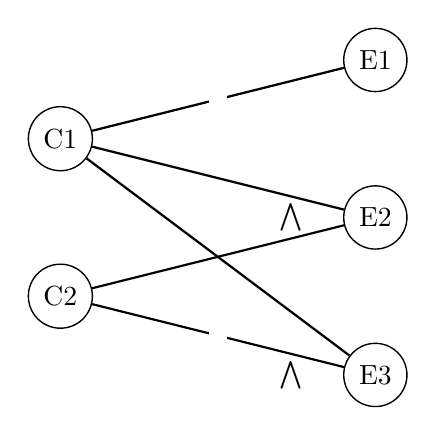
\begin{tikzpicture}
        \GraphInit[vstyle=Normal]
        \Vertex[x=0, y=3]{C1}
        \Vertex[x=0, y=1]{C2}
        \Vertex[x=4, y=0]{E3}
        \Vertex[x=4, y=2]{E2}
        \Vertex[x=4, y=4]{E1}
        \Edge[label=$\thicksim$](C1)(E1)
        \Edge[label=$\thicksim$](C2)(E3)
        \Edge(C1)(E2)
        \Edge(C1)(E3)
        \Edge(C2)(E2)
        \draw (E2) node[left=0.8cm]{$\bigwedge$};
        \draw (E3) node[left=0.8cm]{$\bigwedge$};
    \end{tikzpicture}
    \caption{Cause-and-effect graph for the previously defined rules.}
    \label{fig:cause-n-effect-graph}
\end{figure}

The cause-and-effect graph can be very hard to deal with if specifications are complex enough. Because of that, the tester should convert the graph to a decision table after developing the cause-and-effect graph. This way the test cases can be inferred from the decision table instead of the graph.

\section{Decision Tables}
The decision table shows the effects of all possible combinations of causes. Each column in the decision table represents a test case and lists each combination of causes. Each row represents a cause and effect. The entries of the decision table can be a "1" for a cause or effect that is present, a "0" to represent the absence of a cause or effect, and "---" to indicate a \emph{"don't care"} value.

\begin{table}[H]
    \centering
    \renewcommand{\arraystretch}{1.2}
    \caption{Decision table for the previously defined cause-and-effect graph.}
    \label{tab:decision-table}
    \begin{tabular*}{\textwidth}{l @{\extracolsep{\fill}} llll}
        \toprule
         & \thead{T1} & \thead{T2} & \thead{T3}\\
        \midrule
        C1 & 1 & 1 & 0\\
        C2 & 1 & 0 & ---\\
        \midrule
        E1 & 0 & 0 & 1\\
        E2 & 1 & 0 & 0\\
        E3 & 0 & 1 & 0\\
        \bottomrule
    \end{tabular*}
\end{table}

The problem with decision tables is that there might be many causes and effects to consider for a complex specification. In those cases, the tester can decompose the specification into lower-level units. Then, (s)he develops cause-and-effect graphs and decision tables for these.

\section{Error Guessing}
Error guessing is based on the tester's past experience. The tester's experience with code similar to the code-under-test greatly helps her/him to find the defects. Some examples of defects that can be found by error guessing might be division by zero or conditions around array boundaries.

\section{Exercises}

\begin{exercise}
    Bank account can be 500 to 1000 for special customers,  0 to 499 for ordinary customers, 2000 for companies (the field type is integer).
    
    \begin{enumerate}[a),noitemsep]
        \item What are the equivalence classes?
        \item Fill the Table \ref{tab:ex10-question-b} by finding appropriate test cases for the equivalence classes you found in previous question (a). \emph{Add lines if necessary.}
        \item Fill the Table \ref{tab:ex10-question-c} by finding appropriate test cases for the boundary testing method. \emph{Add lines if necessary.}
    \end{enumerate}
    
    \begin{table}[H]
        \centering
        \renewcommand{\arraystretch}{1.2}
        \caption{Test cases for equivalence classes.}
        \label{tab:ex10-question-b}
        \begin{tabularx}{\textwidth}{llXX}
            \toprule
            \thead{Test Case \#} & \thead{Value} & \thead{Equivalence Classes} & \thead{Result (Val./Inval.)}\\
            \midrule
            1 & & & \\
            2 & & & \\
            3 & & & \\
            4 & & & \\
            5 & & & \\
            6 & & & \\
            7 & & & \\
            8 & & & \\
            9 & & & \\
            10 & & & \\
            11 & & & \\
            12 & & & \\
            13 & & & \\
            14 & & & \\
            \bottomrule
        \end{tabularx}
    \end{table}
    
    \begin{table}[H]
    \centering
    \renewcommand{\arraystretch}{1.2}
    \caption{Test cases for BVA strategy.}
    \label{tab:ex10-question-c}
        \begin{tabularx}{\textwidth}{llX}
            \toprule
            \thead{Test Case \#} & \thead{Value} & \thead{Result (Valid/Invalid)}\\
            \midrule
            1 & & \\
            2 & & \\
            3 & & \\
            4 & & \\
            5 & & \\
            6 & & \\
            7 & & \\
            8 & & \\
            9 & & \\
            10 & & \\
            11 & & \\
            12 & & \\
            13 & & \\
            14 & & \\
            \bottomrule
        \end{tabularx}
    \end{table}
\end{exercise}

\begin{solution}
    Answer for the item a):
    
    \begin{itemize}[noitemsep]
        \item Valid Classes
        \begin{itemize}[noitemsep]
            \item (Special) $\rightarrow$ [500, 1000]
            \item (Ordinary) $\rightarrow$ [0, 499]
            \item (Company) $\rightarrow$ 2000
        \end{itemize}
        \item Invalid Classes
        \begin{itemize}[noitemsep]
            \item (Special) $\rightarrow$ $(-\infty, 499] \cup [1001, \infty)$
            \item (Ordinary) $\rightarrow$ $(-\infty, -1] \cup [500, \infty)$
            \item (Company) $\rightarrow$ $(-\infty, 1999] \cup [2001, \infty)$
        \end{itemize}
    \end{itemize}
    
    Answer for the item b):
    
    \begin{table}[H]
    \centering
    \renewcommand{\arraystretch}{1.2}
    \caption{Suggested test cases for equivalence classes.}
    \label{tab:ex10-solution-b}
        \begin{adjustbox}{max width=\textwidth}
            \begin{tabular}{llll}
                \toprule
                \thead{Test Case \#} & \thead{Value} & \thead{Equivalence Classes} & \thead{Result (Valid/Invalid)}\\
                \midrule
                1 & 600 & (Special) $\rightarrow$ [500, 1000] & Valid\\
                2 & 300 & (Ordinary) $\rightarrow$ [0, 499] & Valid\\
                3 & 2000 & (Company) $\rightarrow$ 2000 & Valid\\
                4 & 2500 & (Special) $\rightarrow$ $(-\infty, 499] \cup [1001, \infty)$ & Invalid\\
                5 & -10 & (Ordinary) $\rightarrow$ $(-\infty, -1] \cup [500, \infty)$ & Invalid\\
                6 & 1000 & (Company) $\rightarrow$ $(-\infty, 1999] \cup [2001, \infty)$ & Invalid\\
                \bottomrule
            \end{tabular}
        \end{adjustbox}
    \end{table}
    
    \begin{table}[H]
    \centering
    \renewcommand{\arraystretch}{1.2}
    \caption{Suggested test cases for BVA strategy.}
    \label{tab:ex10-solution-c}
        \begin{tabular*}{\textwidth}{l @{\extracolsep{\fill}} lll}
            \toprule
            \thead{Test Case \#} & \thead{Value} & \thead{Result (Valid/Invalid)}\\
            \midrule
            1 & 499 & Invalid\\
            2 & 500 & Valid\\
            3 & 501 & Valid\\
            4 & 999 & Valid\\
            5 & 1000 & Valid\\
            6 & 1001 & Invalid\\
            7 & -1 & Invalid\\
            8 & 0 & Valid\\
            9 & 1 & Valid\\
            10 & 499 & Valid\\
            11 & 500 & Invalid\\
            12 & 501 & Invalid\\
            \bottomrule
        \end{tabular*}
    \end{table}
\end{solution}

\begin{exercise}
    The following is the interface of a function called \lstinline!ConvertIntToString! in the Java language.
    
    The requirements (pre-condition and post-condition) of the function are as follows:
    \begin{itemize}[noitemsep]
        \item \textbf{Pre-condition:} input is a valid int
        \item \textbf{Post-condition:} return a string corresponding to the input integer value, e.g., return string value of "-9231" for integer value of -9231. Return NULL if input is an invalid integer
    \end{itemize}

    Choose an appropriate black-box technique (equivalence class partitioning, boundary value analysis) to derive test cases for this function. Note that each test case should have a concrete input value for input \lstinline!int! and the expected output \lstinline!String!. You should use the following format for the list of your test cases.
    
    \begin{enumerate}[a),noitemsep]
        \item What are the equivalence classes? Fill the Table \ref{tab:ex11-question-a} by finding appropriate test cases for the equivalence classes.
        \begin{itemize}[noitemsep]
            \item Valid Classes:
            \item Invalid Classes:
        \end{itemize}
        \item Fill the Table \ref{tab:ex11-question-b} by finding appropriate test cases for the boundary testing method. \emph{Add lines if necessary.}
    \end{enumerate}

    \begin{table}[H]
    \centering
    \renewcommand{\arraystretch}{1.2}
    \caption{Test cases for equivalence classes.}
    \label{tab:ex11-question-a}
        \begin{tabular*}{\textwidth}{l @{\extracolsep{\fill}} llll}
            \toprule
            \thead{Test Case \#} & \thead{Value} & \thead{Equivalence Classes} & \thead{Result (Valid/Invalid)}\\
            \midrule
            1 & & & \\
            2 & & & \\
            3 & & & \\
            4 & & & \\
            \bottomrule
        \end{tabular*}
    \end{table}
    
    \begin{table}[H]
    \centering
    \renewcommand{\arraystretch}{1.2}
    \caption{Test cases for BVA strategy.}
    \label{tab:ex11-question-b}
        \begin{tabular*}{\textwidth}{l @{\extracolsep{\fill}} lll}
            \toprule
            \thead{Test Case \#} & \thead{Value} & \thead{Result (Valid/Invalid)}\\
            \midrule
            1 & & \\
            2 & & \\
            3 & & \\
            4 & & \\
            \bottomrule
        \end{tabular*}
    \end{table}
    
    \begin{lstlisting}[caption={The implementation of the program that should not supposed to be known.}]
public class IntToString {
    public static String ConvertIntToString(int number) {
        int StringConvert = 48;
        int eachDigit = number;
        int afterDivide = number;
        String reVal = "";
        
        while (afterDivide > 0) {
            eachDigit = afterDivide % 10;
            afterDivide = afterDivide / 10;
            if(eachDigit == 0) {
                reVal += "0";
            }
            else if(eachDigit == 1) {
                reVal += "1";
            }
            else if(eachDigit == 2) {
                reVal += "2";
            }
            else if(eachDigit == 3) {
                reVal += "3";
            }
            else if(eachDigit == 4) {
                reVal += "4";
            }
            else if(eachDigit == 5) {
                reVal += "5";
            }
            else if(eachDigit == 6) {
                reVal += "6";
            }
            else if(eachDigit == 7) {
                reVal += "7";
            }
            else if(eachDigit == 8) {
                reVal += "8";
            }
            else if(eachDigit == 9) {
                reVal += "9";
            }
        }
        String reVal2 = "";
        for (int index = reVal.length() -1 ; index >= 0 ; index--) {
            reVal2 += reVal.charAt(index);
        }
        return reVal2;
    }
}
    \end{lstlisting}
\end{exercise}

\begin{solution}
    Answer for the item a):
    
    \begin{itemize}[noitemsep]
        \item \textbf{Valid Classes:} (-inf, +inf) instance of integer
        \item \textbf{Invalid Classes:} String, (-inf, +inf) floating point numbers, boolean, Objects
    \end{itemize}
    
    \begin{table}[H]
    \centering
    \renewcommand{\arraystretch}{1.2}
    \caption{Suggested test cases for equivalence classes.}
    \label{tab:ex11-solution-a}
         \begin{tabular*}{\textwidth}{l @{\extracolsep{\fill}} llll}
            \toprule
            \thead{Test Case \#} & \thead{Value} & \thead{Equivalence Classes} & \thead{Result (Valid/Invalid)}\\
            \midrule
            1 & 4785 & (-inf, +inf) instance of integer & Valid\\
            2 & \lstinline!"hello"! & String & Invalid\\
            3 & 45.5 & Floating point & Invalid\\
            4 & \lstinline!'c'! & char & Invalid\\
            \bottomrule
        \end{tabular*}
    \end{table}
    
    Answer for the item b):
    \begin{table}[H]
    \centering
    \renewcommand{\arraystretch}{1.2}
    \caption{Suggested test cases for BVA strategy.}
    \label{tab:ex11-solution-b}
        \begin{tabular*}{\textwidth}{l @{\extracolsep{\fill}} lll}
            \toprule
            \thead{Test Case \#} & \thead{Value} & \thead{Result (Valid/Invalid)}\\
            \midrule
            1 & -2147483649 & Invalid\\
            2 & -2147483648 & Valid\\
            3 & 2147483647 & Valid\\
            4 & 2147483648 & Invalid\\
            \bottomrule
        \end{tabular*}
    \end{table}
\end{solution}

\begin{exercise}
    The program accepts three integers, a, b, and c as inputs. These are taken to be sides of the triangle. The integers a, b, and c must satisfy following conditions:
    
    \begin{enumerate}[label=\textbf{Condition \arabic*:},left=0pt,noitemsep]
        \item $1 \le a \le 200$
        \item $1 \le b \le 200$
        \item $1 \le c \le 200$
        \item $a < b + c$
        \item $b < a + c$
        \item $c < a + b$
    \end{enumerate}
    
    The output of the program is the type of triangle determined by the three sides: Equilateral, Isosceles, Scalene, or NotATriangle. If an input value fails any of conditions Condition 1, Condition 2 or Condition 3, the program notes this with an output message such as "Value of b is not in the range of permitted values." If values of a, b, and c satisfy Condition 4, Condition 5, and Condition 6, one of four mutually exclusive outputs is given:
    
    \begin{enumerate}[nosep]
        \item If all three sides are equal, the program output is Equilateral.
        \item If exactly one pair of sides is equal, the program output is Isosceles.
        \item If no pair of sides is equal, the program output is Scalene.
        \item If any of conditions Condition 4, Condition 5, and Condition 6 is not met, the program output is NotATriangle.
    \end{enumerate}
    
    Test the program with Decision Table-Based testing method by doing followings \autocite{jorgensen2013software}:
    \begin{enumerate}[label=\alph*),nosep]
        \item Draw the Cause-and-effect graph.
        \item Create a decision table for the problem.
        \item Create test cases.
        \item Run all test cases and write which ones are passed and which ones are failed.
    \end{enumerate}
\end{exercise}

\begin{solution}
    Answer for the item a):
    
    To draw a cause-and-effect graph, all the causes and effects should be extracted by elaborating the specification.
    
    \begin{enumerate}[nosep]
        \item[\textbf{C1:}] The given side lengths permit to build a triangle.
        \item[\textbf{C2:}] The length of side a is equal to side b.
        \item[\textbf{C3:}] The length of side b is equal to side c.
        \item[\textbf{C4:}] The length of side a is equal to side c.
        \item[\textbf{E1:}] The lengths allow to build a equilateral triangle.
        \item[\textbf{E2:}] The lengths allow to build a isosceles triangle.
        \item[\textbf{E3:}] The lengths allow to build a scalene triangle.
        \item[\textbf{E4:}] It is impossible.
        \item[\textbf{E5:}] With the given lengths, it is impossible to form a triangle.
    \end{enumerate}
    
    \begin{figure}[H]
        \centering
        \begin{tabular}{iii}
            exercise-12a-solution1 & exercise-12a-solution2 & exercise-12a-solution3\\
            exercise-12a-solution4 & exercise-12a-solution5 & exercise-12a-solution6
        \end{tabular}
        \caption{Cause-and-effect graph for the question.}
        \label{fig:cne-graphs}
    \end{figure}
    
    Answer for the item b):
    
    \begin{table}[H]
        \centering
        \renewcommand{\arraystretch}{1.2}
        \caption{Decision table for the previously defined cause-and-effect graph.}
        \label{tab:sol12-decision-table}
        \begin{tabularx}{\textwidth}{l|XXXXXXXXX}
            \toprule
             & \thead{T1} & \thead{T2} & \thead{T3} & \thead{T4} & \thead{T5} & \thead{T6} & \thead{T7} & \thead{T8} & \thead{T9}\\
            \midrule
            C1: Triangle & 0 & 1 & 1 & 1 & 1 & 1 & 1 & 1 & 1\\
            C2: a=b? & --- & 1 & 1 & 1 & 1 & 0 & 0 & 0 & 0\\
            C3: b=c? & --- & 1 & 1 & 0 & 0 & 1 & 1 & 0 & 0\\
            C4: a=c? & --- & 1 & 0 & 1 & 0 & 1 & 0 & 1 & 0\\
            \midrule
            E1: Equilateral & 0 & 1 & 0 & 0 & 0 & 0 & 0 & 0 & 0\\
            E2: Isosceles & 0 & 0 & 0 & 0 & 1 & 0 & \colorbox{red}{1} & \colorbox{red}{1} & 0\\
            E3: Scalene & 0 & 0 & 0 & 0 & 0 & 0 & 0 & 0 & \colorbox{red}{1}\\
            E4: Impossible & 0 & 0 & 1 & 1 & 0 & 1 & 0 & 0 & 0\\
            E5: Not a Triangle & 1 & 0 & 0 & 0 & 0 & 0 & 0 & 0 & 0\\
            \bottomrule
        \end{tabularx}
    \end{table}
    
    Answer for the item c):
    
    \begin{enumerate}[label=\textbf{Test \arabic*:},left=0pt,nosep]
        \item $a=1, b=2, c=7 \rightarrow E5$
        \item $a=3, b=3, c=3 \rightarrow E1$
        \item $a=2, b=2, c=3 \rightarrow E2$
        \item $a=3, b=2, c=2 \rightarrow E2$
        \item $a=2, b=3, c=2 \rightarrow E2$
        \item $a=3, b=4, c=5 \rightarrow E3$
    \end{enumerate}
    
    Answer for the item d):
    
    The red marked test cases in Table \ref{tab:sol12-decision-table} are failed tests.
\end{solution}
    \chapter{Selenium for Black-Box Testing Strategies}
Selenium, with its official name "The Selenium Browser Automation Project" is an umbrella project for various tools and libraries that automates certain web browser tasks by their definition in the official website\footnote{\url{https://www.selenium.dev/documentation/}}. Selenium is a gateway to access browser features from a programming language through various language bindings. It presents a consistent API to access those features. An example that opens the official Selenium website is given in Listing \ref{lst:selenium-example} with Java programming language.

\begin{lstlisting}[caption={A Java program that opens the official Selenium website through a Chrome-based browser.}, label=lst:selenium-example]
import org.openqa.selenium.WebDriver;
import org.openqa.selenium.chrome.ChromeDriver;

public class HelloSelenium {
    public static void main(String[] args) {
        WebDriver driver = new ChromeDriver();

        driver.get("https://selenium.dev");

        driver.quit();
    }
}
\end{lstlisting}

At its core Selenium has a WebDriver. Once it has been installed, all Chromium and Gecko-based browsers can be controlled with a few lines of code through six different programming languages. One of these programming languages is not surprisingly Java. In this section, installation steps and a few examples to introduce the basics of Selenium are covered.

\section{Installation}
There are two ways to work with Selenium. With the first one, you have to install the language bindings libraries for your language of choice, the browser you want to use, and the driver for that browser. This is the seemingly more professional way to work with Selenium. The other way to work is to install the Selenium IDE\footnote{\url{https://www.selenium.dev/selenium-ide/}}. Selenium IDE provides a record-and-replay style of workflow. It is easier to work with and it is not required to write code.

It is easy to install the Selenium library for Java with Maven. Just add the Selenium dependency which is shown in the code snippet in Listing \ref{lst:selenium-dep}.

\begin{lstlisting}[language=XML,caption={The Selenium dependency for Maven.},label=lst:selenium-dep]
<dependency>
  <groupId>org.seleniumhq.selenium</groupId>
  <artifactId>selenium-java</artifactId>
  <version>4.0.0</version>
</dependency>
\end{lstlisting}

After that, the WebDriver of choice should be installed. Notice that the major version number of the WebDriver must match with the major version number of the installed browser. All WebDriver utilities are provided by the vendor themselves and should be downloaded from their official websites\footnote{\url{https://www.selenium.dev/documentation/webdriver/getting\_started/install\_drivers/}}. The installed WebDriver should be visible on PATH. Each operating system has a different way to maintain PATH. In Linux, no further action is needed since most package managers automatically create symbolic links to the directories which are scanned by default. Alternatively, it is possible to use the installed driver by hard-coding the driver path. Example of it is given in the code snippet in Listing \ref{lst:selenium-hc-path}.

\begin{lstlisting}[caption={Using the driver from a hard-coded path.},label=lst:selenium-hc-path]
System.setProperty("webdriver.chrome.driver","/path/to/chromedriver");
ChromeDriver driver = new ChromeDriver();
\end{lstlisting}

\section{Usage}
In this section, it is assumed that Google Chrome is the choice of browser. Therefore, Chrome WebDriver should be installed. After installing the Selenium library, the browser, and the relevant WebDriver, you can open the Selenium-controlled browser with the following code snippet.

\begin{lstlisting}[caption={Start a Selenium-controlled browser instance.}]
ChromeOptions options = new ChromeOptions();
driver = new ChromeDriver(options);

driver.quit();
\end{lstlisting}

By default, Selenium 4 is compatible with Chrome v75 and greater. Note that the version of the Chrome browser and the version of chromedriver must match the major version. In addition to the shared capabilities, there are specific Chrome capabilities that can be used. Let's break down and extend the code.

The following code snippet opens a Selenium-controlled browser instance with default options.
\begin{lstlisting}
WebDriver driver = new ChromeDriver();
\end{lstlisting}

This code snippet opens the given web page on the browser.
\begin{lstlisting}
driver.get("https://selenium.dev");
\end{lstlisting}

One can access all of the attributes about an opened web page through the driver variable. In the following code snippet, the title of the web page is accessed.
\begin{lstlisting}
driver.getTitle(); // => "Google"
\end{lstlisting}

Synchronizing the code with the current state of the browser is one of the biggest challenges with Selenium, and doing it well is an advanced topic. Essentially you want to make sure that the element is on the page before you attempt to locate it and the element is in an interactable state before you attempt to interact with it. An implicit wait is rarely the best solution, but it’s the easiest to demonstrate here, so we’ll use it as a placeholder.
\begin{lstlisting}
driver.manage().timeouts().implicitlyWait(Duration.ofMillis(500));
\end{lstlisting}

The majority of commands in most Selenium sessions are element related, and you can’t interact with one without first finding an element.
\begin{lstlisting}
WebElement searchBox = driver.findElement(By.name("q"));
WebElement searchButton = driver.findElement(By.name("btnK"));
\end{lstlisting}

There are only a handful of actions to take on an element, but you will use them frequently.
\begin{lstlisting}
searchBox.sendKeys("Selenium");
searchButton.click();
\end{lstlisting}

Elements store a lot of information that can be requested. Notice that we need to relocate the search box because the DOM has changed since we first located it.
\begin{lstlisting}
driver.findElement(By.name("q")).getAttribute("value"); // => "Selenium"
\end{lstlisting}

This ends the driver process, which by default closes the browser as well. No more commands can be sent to this driver instance.
\begin{lstlisting}
driver.quit();
\end{lstlisting}

Let’s combine these previous things into a complete script.
\begin{lstlisting}
import org.openqa.selenium.By;
import org.openqa.selenium.WebDriver;
import org.openqa.selenium.WebElement;
import org.openqa.selenium.chrome.ChromeDriver;

public class HelloSelenium {
    public static void main(String[] args) {
        driver = new ChromeDriver();

        driver.get("https://google.com");
        
        driver.getTitle(); // => "Google"

        driver.manage().timeouts().implicitlyWait(Duration.ofMillis(500));
        
        WebElement searchBox = driver.findElement(By.name("q"));
        WebElement searchButton = driver.findElement(By.name("btnK"));
        
        searchBox.sendKeys("Selenium");
        searchButton.click();
        
        searchBox = driver.findElement(By.name("q"));
        searchBox.getAttribute("value"); // => "Selenium"
        
        driver.quit();
    }
\end{lstlisting}

WebDriver drives a browser natively, as a user would, either locally or on a remote machine using the Selenium server, marks a leap forward in terms of browser automation. More information on the API can be found in the documentation\footnote{\url{https://www.selenium.dev/documentation/webdriver/}}.

Several configuration changes need to be made to run the program from the \lstinline!main(String[])! function. The first one is to add the fully qualified class name of the class that contains the main function. It is marked as \lstinline!mainClass! variable in the \lstinline!pom.xml! file. Add the following code snippet inside of the \lstinline[language=XML]!<properties>! element after the compiler target element:
\begin{lstlisting}[language=XML]
<exec.mainClass>the.package.name.HelloSelenium</exec.mainClass>
\end{lstlisting}

Here, the package name can be nothing or the package name that is indicated at the first line of the main class. Now, we need to tell Eclipse to build and run the program without running the tests when we send the command Maven build. If tests are run after a successful build, make sure that they all pass. Otherwise, the build will fail.

To create a build and run without tests config, right-click to the project. From the context menu, choose \menu{Run As > Run Configurations...}. A dialog box should appear. In the dialog, right-click to the Maven Build and choose \menu{New Configuration}. This should create a configuration similar to Figure \ref{fig:run-configs}. In the Goals textbox, write \lstinline[language={}]!clean install exec:java!. Finally, tick the \lstinline[language={}]!Skip Tests! checkbox. Click \emph{Apply}, then \emph{Run} buttons. If everything works correctly, a browser window should appear and search for "Selenium" in Google, and close.

\begin{figure}[H]
    \centering
    \includegraphics[width=\textwidth]{images/maven-run-config.png}
    \caption{Run configurations dialog window.}
    \label{fig:run-configs}
\end{figure}

\section{Complete Examples}
The aim here is to write a program that tests another program that the tester has no idea of its code. Selenium's API can be thought of as instructions for a browser that performs the tests. First, the tester must make the test plan. Then, (s)he prepares the test cases. Finally, the test cases are converted into a Java program that is written with Selenium API to instruct the browser to perform the tests.
    
    \appendix
    \chapter{XML Path Language (XPath)}
\label{ch:appendix-xpath}
XPath is a query language to search nodes in a markup language like XML. In XPath, we write path expressions to identify certain nodes in the document \autocite{elmasri2014}. Generally, XPath returns either values (from leaf nodes), elements, or attributes. The names that appear in an XPath are the node names, attribute names, or additional qualifier conditions. There are two separators in XPath. A single slash (/) appears before a tag means that the tag must be a direct child of its parent. A single slash (//) means that the tag can appear as a descendant of the previous tag at any level. Several examples are given below:

\begin{lstlisting}[language={},caption={Several examples of XPath from Elmasri et al..}]
/company
/company/department
//employee[employeeSalary gt 70000]/employeeName
/company/employee[employeeSalary gt 70000]/employeeName
/company/project/projectWorker[hours ge 20.0]
\end{lstlisting}

The expression in line (1) finds the company root node and returns all of its descendants including itself (a.k.a. all of the XML document). XPath can also contain the filename information as well. For example, suppose that the XML file is in a remote location such as \lstinline[language={}]!www.company.com/info.xml!. Then, we can get the company root node via XPath \lstinline[language={}]!doc(www.company.com/info.xml)/company!.

The expression in line (2) returns all department elements and their descendent subtrees. The order of the returned elements follows the exact order that they appear on the XML document. If we do not know the full path to a specific element, // is the convenient way to find it. The expression in line (3) is such an example. It searches and finds an element called \lstinline[language={}]!employee! and checks if the value of its child element \lstinline[language={}]!employeeSalary! is greater than 70000. If so, it returns its child called \lstinline[language={}]!employeeName!. The following expression in line (4) is the same one as the previous one except in line (4) the full path is specified. In the last example, at line (5),  the XPath returns all \lstinline[language={}]!projectWorker! elements and their children which has an hours child element whose value is greater than or equal to 20.0.

In XPath, we can use wildcards (*). A wildcard means that all of the elements regardless of their types. For example, \lstinline[language={}]!/company/*! query returns all the elements under the root note \lstinline[language={}]!company!. If we want to address an attribute of a node, we use @ symbol. For instance, the \lstinline[language={}]!//title[@lang='en']! expression returns any title element that has a \lstinline[language={}]!lang! attribute is set to the string \lstinline[language={}]!en!.
    
    \backmatter
    \printbibliography[heading=bibintoc]
\end{document}
